В третьей главе рассматривается практическая реализация генератора данных
TPC-H~\cite{schengen-repo}. Здесь основное внимание уделяется тому,
как устроены формирование табличных данных, подготовка колонoчных батчей,
запись результата в разные форматы и использование генератора как встроенного
источника данных.

\subsection{Реализация генерации таблиц}

\subsubsection{Организация генерации по партициям}

Реализация генерации начинается с выбора требуемых таблиц и подготовки общего
текстового пула. После этого для каждой таблицы формируется набор логических
партиций, а для каждой партиции создается собственный контекст генерации с
диапазоном строк, масштабом генерации и параметрами размера батча.
При запуске обработки партиции внутренние генераторы сразу переводятся к
началу нужного диапазона строк, после чего партиция выдает последовательность
колонoчных батчей. Каждый батч сохраняет положение своего первого ряда в
таблице, поэтому несколько рабочих потоков могут параллельно строить батчи
разных партиций и передавать их в следующий слой без потери локального порядка
строк.

\subsubsection{Генерация значений и использование текстового пула}

Для числовых атрибутов используются ограниченные генераторы целых значений.
Они применяются для количеств, балансов, скидок, налогов, датовых смещений и
других величин, для которых спецификацией TPC-H задан конечный
диапазон допустимых значений. Для больших диапазонов ключей используется
расширенный вариант генерации, допускающий работу с 64-разрядными значениями.

Для строковых атрибутов применяются несколько способов формирования значения.
Значения из фиксированных словарей, например сегменты рынка, приоритеты
заказов, типы деталей, инструкции отгрузки и режимы доставки, выбираются из
взвешенных распределений. Имена деталей формируются как последовательности
токенов, а адреса строятся как алфавитно-цифровые строки переменной длины.
Телефонные номера вычисляются из ключа страны и случайных локальных компонент.

Генерация текстовых атрибутов в TPC-H задается набором распределений
из файла \texttt{dists.dss}~\cite{tpch-spec,dbgen-mirror}. Каждый блок содержит
имя распределения и число элементов \texttt{COUNT}. Далее приводится список
токенов с соответствующими весами; вес определяет относительную частоту выбора
токена.

\begin{lstlisting}[style=reportdss,caption={Общий вид распределения},label={lst:chapter3-dss-format}]
# <token> | <weight> # comment

BEGIN articles
COUNT|3
the|50
a|20
an|5
END articles
\end{lstlisting}

Пусть распределение содержит токены $t_i$ с весами $w_i$, а
\begin{equation}
    W = \sum_{i=1}^{n} w_i.
\end{equation}
Тогда выбирается случайное число $u \in [0, W)$, и возвращается первый токен
$t_j$, для которого выполнено условие
\begin{equation}
    \sum_{i=1}^{j} w_i > u.
\end{equation}
Именно эта схема накопления весов используется при выборе значений из словарей.

Распределение \texttt{grammar} задает верхнеуровневую схему предложения.
Символы \texttt{N}, \texttt{V}, \texttt{P} и \texttt{T} обозначают именную
группу, глагольную группу, предложную группу и знак завершения предложения.

\begin{lstlisting}[style=reportdss,caption={Верхнеуровневая грамматика предложения},label={lst:chapter3-dss-grammar}]
###
# grammar
# first level grammar. N=noun phrase, V=verb phrase,
# P=prepositional phrase, T=sentence termination
##
BEGIN grammar
COUNT|5
N V T|3
N V P T|3
N V N T|3
N P V N T|1
N P V P T|1
END grammar
\end{lstlisting}

Далее нетерминальные символы раскрываются через распределения \texttt{np} и
\texttt{vp}, которые определяют внутреннюю форму именной и глагольной групп.

\begin{lstlisting}[style=reportdss,caption={Раскрытие именной и глагольной групп},label={lst:chapter3-dss-np-vp}]
###
# NP
BEGIN np
COUNT|4
N|10
J N|20
J, J N|10
D J N|50
END np

###
# VP
BEGIN vp
COUNT|4
V|30
X V|1
V D|40
X V D|1
END vp
\end{lstlisting}

Терминальные символы подставляются из словарей отдельных частей речи, например
\texttt{nouns} и \texttt{verbs}.

\begin{lstlisting}[style=reportdss,caption={Словари терминальных токенов},label={lst:chapter3-dss-terminals}]
BEGIN nouns
COUNT|45
packages|40
requests|40
accounts|40
deposits|40
foxes|20
ideas|20
END nouns

BEGIN verbs
COUNT|40
sleep|20
wake|20
are|20
cajole|20
haggle|20
END verbs
\end{lstlisting}

Из получаемых предложений заранее формируется текстовый пул - общий
текстовый буфер. При генерации конкретного комментария программа выбирает в нем
смещение и длину фрагмента, после чего использует соответствующий срез как
значение атрибута. Такой подход уменьшает накладные расходы при генерации
длинных текстовых полей. Для некоторых таблиц, например supplier,
поверх выбранного текста дополнительно может применяться модификация по правилу
BBB\footnote{Правило BBB применяется при формировании
атрибута \texttt{s\_comment} таблицы \texttt{supplier}: в текст комментария
вставляется подстрока <<Customer Complaints>> или
<<Customer Recommends>>~\cite{tpch-spec}.}, предусмотренному спецификацией
TPC-H~\cite{tpch-spec}.

\begin{figure}[H]
\centering
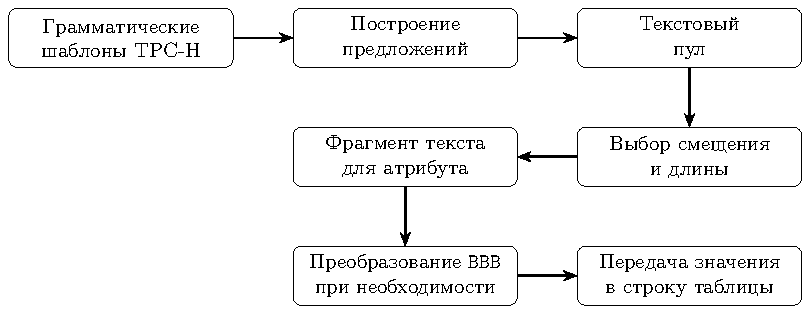
\includegraphics[width=0.92\textwidth]{../expl-note/image/textpool-diagram.pdf}
\caption{Схема формирования текстовых атрибутов на основе пула текста}
\label{fig:chapter3-textpool-flow}
\end{figure}

\subsubsection{Формирование таблиц набора данных}

Для каждой таблицы используется собственный генератор, реализующий правила
формирования ключей и зависимых атрибутов, заданные спецификацией
TPC-H.

\renewcommand{\arraystretch}{1.1}

\paragraph{Таблица region}
\begin{center}
\small
\begin{tabular}{|p{0.18\textwidth}|p{0.10\textwidth}|p{0.58\textwidth}|}
\hline
\textbf{Атрибут} & \textbf{Ключ} & \textbf{Правило формирования} \\
\hline
\texttt{r\_regionkey} & PK & Последовательная нумерация строк, начиная с нуля. \\
\hline
\texttt{r\_name} &  & Выбирается из фиксированного справочника регионов TPC-H. \\
\hline
\texttt{r\_comment} &  & Выбирается из текстового пула. \\
\hline
\end{tabular}
\end{center}

\noindent Символическая запись генератора region приведена в
приложении \ref{appendix:region}.

\paragraph{Таблица nation}
\begin{center}
\small
\begin{tabular}{|p{0.18\textwidth}|p{0.10\textwidth}|p{0.58\textwidth}|}
\hline
\textbf{Атрибут} & \textbf{Ключ} & \textbf{Правило формирования} \\
\hline
\texttt{n\_nationkey} & PK & Последовательная нумерация строк, начиная с нуля. \\
\hline
\texttt{n\_name} &  & Выбирается из предопределенного справочника наций. \\
\hline
\texttt{n\_regionkey} & FK & Вычисляется по таблице наций и весам распределения регионов, заданным спецификацией TPC-H. \\
\hline
\texttt{n\_comment} &  & Выбирается из текстового пула. \\
\hline
\end{tabular}
\end{center}

\noindent Символическая запись генератора nation приведена в
приложении \ref{appendix:nation}.

\paragraph{Таблица supplier}
\begin{center}
\small
\begin{tabular}{|p{0.18\textwidth}|p{0.10\textwidth}|p{0.58\textwidth}|}
\hline
\textbf{Атрибут} & \textbf{Ключ} & \textbf{Правило формирования} \\
\hline
\texttt{s\_suppkey} & PK & Номер строки с единичным смещением. \\
\hline
\texttt{s\_name} &  & Формируется по шаблону \texttt{Supplier\#\%09d}. \\
\hline
\texttt{s\_address} &  & Формируется как алфавитно-цифровая строка переменной длины. \\
\hline
\texttt{s\_nationkey} & FK & Выбирается из допустимого диапазона ключей наций. \\
\hline
\texttt{s\_phone} &  & Вычисляется из ключа страны и случайных локальных компонент. \\
\hline
\texttt{s\_acctbal} &  & Генерируется как ограниченное числовое значение и переводится в денежный формат. \\
\hline
\texttt{s\_comment} &  & Выбирается из текстового пула; при выполнении условия может модифицироваться по правилу BBB. \\
\hline
\end{tabular}
\end{center}

\noindent Символическая запись генератора supplier приведена в
приложении \ref{appendix:supplier}.

\paragraph{Таблица part}
\begin{center}
\small
\begin{tabular}{|p{0.18\textwidth}|p{0.10\textwidth}|p{0.58\textwidth}|}
\hline
\textbf{Атрибут} & \textbf{Ключ} & \textbf{Правило формирования} \\
\hline
\texttt{p\_partkey} & PK & Последовательная нумерация строк с единичным смещением. \\
\hline
\texttt{p\_name} &  & Формируется как последовательность токенов из словаря цветов. \\
\hline
\texttt{p\_mfgr} &  & Строится по номеру производителя. \\
\hline
\texttt{p\_brand} &  & Вычисляется по номеру производителя и дополнительному номеру бренда. \\
\hline
\texttt{p\_type} &  & Выбирается из словаря типов деталей. \\
\hline
\texttt{p\_size} &  & Генерируется из ограниченного числового диапазона. \\
\hline
\texttt{p\_container} &  & Выбирается из словаря контейнеров. \\
\hline
\texttt{p\_retailprice} &  & Детерминированно вычисляется по ключу детали. \\
\hline
\texttt{p\_comment} &  & Выбирается из текстового пула. \\
\hline
\end{tabular}
\end{center}

\noindent Символическая запись генератора part приведена в
приложении \ref{appendix:part}.

\paragraph{Таблица partsupp}
\begin{center}
\small
\begin{tabular}{|p{0.18\textwidth}|p{0.10\textwidth}|p{0.58\textwidth}|}
\hline
\textbf{Атрибут} & \textbf{Ключ} & \textbf{Правило формирования} \\
\hline
\texttt{ps\_partkey} & FK & Соответствует текущей детали. \\
\hline
\texttt{ps\_suppkey} & FK & Вычисляется как детерминированное отображение пары <<ключ детали, номер поставщика>>; для каждой детали формируются четыре поставщика. \\
\hline
\texttt{ps\_availqty} &  & Генерируется из ограниченного диапазона доступного количества. \\
\hline
\texttt{ps\_supplycost} &  & Генерируется из ограниченного диапазона и переводится в денежный формат. \\
\hline
\texttt{ps\_comment} &  & Выбирается из текстового пула. \\
\hline
\end{tabular}
\end{center}

\noindent Символическая запись генератора partsupp приведена в
приложении \ref{appendix:partsupp}.

\paragraph{Таблица customer}
\begin{center}
\small
\begin{tabular}{|p{0.18\textwidth}|p{0.10\textwidth}|p{0.58\textwidth}|}
\hline
\textbf{Атрибут} & \textbf{Ключ} & \textbf{Правило формирования} \\
\hline
\texttt{c\_custkey} & PK & Последовательная нумерация строк с единичным смещением. \\
\hline
\texttt{c\_name} &  & Формируется по шаблону \texttt{Customer\#\%09d}. \\
\hline
\texttt{c\_address} &  & Формируется как алфавитно-цифровая строка переменной длины. \\
\hline
\texttt{c\_nationkey} & FK & Выбирается из допустимого диапазона ключей наций. \\
\hline
\texttt{c\_phone} &  & Вычисляется из ключа страны и случайных локальных компонент. \\
\hline
\texttt{c\_acctbal} &  & Генерируется как ограниченное числовое значение и переводится в денежный формат. \\
\hline
\texttt{c\_mktsegment} &  & Выбирается из словаря сегментов рынка. \\
\hline
\texttt{c\_comment} &  & Выбирается из текстового пула. \\
\hline
\end{tabular}
\end{center}

\noindent Символическая запись генератора customer приведена в
приложении \ref{appendix:customer}.

\paragraph{Таблица orders}
\begin{center}
\small
\begin{tabular}{|p{0.18\textwidth}|p{0.10\textwidth}|p{0.58\textwidth}|}
\hline
\textbf{Атрибут} & \textbf{Ключ} & \textbf{Правило формирования} \\
\hline
\texttt{o\_orderkey} & PK & Строится по разреженной схеме из порядкового номера заказа. \\
\hline
\texttt{o\_custkey} & FK & Выбирается из диапазона клиентов с исключением недопустимых ключей. \\
\hline
\texttt{o\_orderstatus} &  & Определяется по числу отгруженных позиций заказа. \\
\hline
\texttt{o\_totalprice} &  & Вычисляется как агрегат по позициям соответствующего заказа. \\
\hline
\texttt{o\_orderdate} &  & Генерируется в допустимом диапазоне дат TPC-H. \\
\hline
\texttt{o\_orderpriority} &  & Выбирается из словаря приоритетов заказов. \\
\hline
\texttt{o\_clerk} &  & Формируется по шаблону \texttt{Clerk\#\%09d}. \\
\hline
\texttt{o\_shippriority} &  & Имеет фиксированное значение \texttt{0}. \\
\hline
\texttt{o\_comment} &  & Выбирается из текстового пула. \\
\hline
\end{tabular}
\end{center}

Символическая запись генератора orders приведена в приложении
\ref{appendix:orders}.

\paragraph{Таблица lineitem}
\begin{center}
\small
\begin{tabular}{|p{0.18\textwidth}|p{0.10\textwidth}|p{0.58\textwidth}|}
\hline
\textbf{Атрибут} & \textbf{Ключ} & \textbf{Правило формирования} \\
\hline
\texttt{l\_orderkey} & FK & Согласован с ключом соответствующего заказа. \\
\hline
\texttt{l\_partkey} & FK & Выбирается из диапазона ключей деталей. \\
\hline
\texttt{l\_suppkey} & FK & Вычисляется по паре <<ключ детали, номер поставщика>>. \\
\hline
\texttt{l\_linenumber} &  & Задает порядковый номер позиции внутри заказа. \\
\hline
\texttt{l\_quantity} &  & Генерируется из ограниченного числового диапазона. \\
\hline
\texttt{l\_extendedprice} &  & Вычисляется по цене детали и количеству. \\
\hline
\texttt{l\_discount} &  & Генерируется как процент скидки из ограниченного диапазона. \\
\hline
\texttt{l\_tax} &  & Генерируется как процент налога из ограниченного диапазона. \\
\hline
\texttt{l\_returnflag} &  & Определяется по отношению даты получения к текущей календарной отметке TPC-H. \\
\hline
\texttt{l\_linestatus} &  & Определяется по отношению даты отгрузки к текущей календарной отметке TPC-H. \\
\hline
\texttt{l\_shipdate} &  & Вычисляется как смещение относительно даты заказа. \\
\hline
\texttt{l\_commitdate} &  & Вычисляется как смещение относительно даты заказа. \\
\hline
\texttt{l\_receiptdate} &  & Вычисляется как смещение относительно даты отгрузки. \\
\hline
\texttt{l\_shipinstruct} &  & Выбирается из словаря инструкций по отгрузке. \\
\hline
\texttt{l\_shipmode} &  & Выбирается из словаря режимов доставки. \\
\hline
\texttt{l\_comment} &  & Выбирается из текстового пула. \\
\hline
\end{tabular}
\end{center}

\noindent Символические записи подготовки диапазона и строки
lineitem приведены в приложении \ref{appendix:lineitem}.

\renewcommand{\arraystretch}{1}

\subsection{Реализация слоя сериализации}

\subsubsection{Общий интерфейс записи}

На этапе реализации слой сериализации принимает готовые колонoчные батчи
Apache Arrow и передает их в драйвер выбранного формата хранения.
Для Parquet и ORC используются файловые компоненты записи,
для Lance и Vortex - мосты во внешний форматный рантайм.
Для локального пути и удаленного URI используется одна и та же схема
размещения результата, поэтому генератору не требуется различать конкретный
тип хранилища.

\subsubsection{Форматы с управляемым стримингом}

Для части форматов с управляемым стримингом, прежде всего Parquet и
ORC, генератор сам управляет тем, как батчи группируются в выходные
артефакты. В этом случае поддерживаются два сценария: раздельная запись
партиций в набор файлов и упорядоченная запись в один итоговый файл. Оба
сценария реализуются внутри слоя сериализации и используют один и тот же
поток готовых батчей.

\begin{lstlisting}[style=reportpseudocode,caption={Выбор режима записи},label={lst:chapter3-write-strategy}]
func deliver_batches(table, batches, output_format, write_strategy):
    strategy = resolve_selected_write_strategy(output_format, write_strategy)

    if strategy == "partition-files":
        return write_partition_files(table, batches, output_format)

    if strategy == "ordered-single-output":
        return write_ordered_single_output(table, batches, output_format)

    return stream_to_native_runtime(table, batches, output_format)
\end{lstlisting}

В режиме раздельной записи партиций каждая партиция записывается независимо,
что естественно сочетается с параллельным формированием данных. В режиме
упорядоченной записи в один итоговый файл батчи от нескольких рабочих потоков
должны быть дополнительно упорядочены перед фиксацией результата. Для этого
используется очередь MPSC (\textit{multi-producer, single-consumer}),
а на стороне потребителя поддерживается буфер готовых партиций.

\begin{figure}[H]
\centering
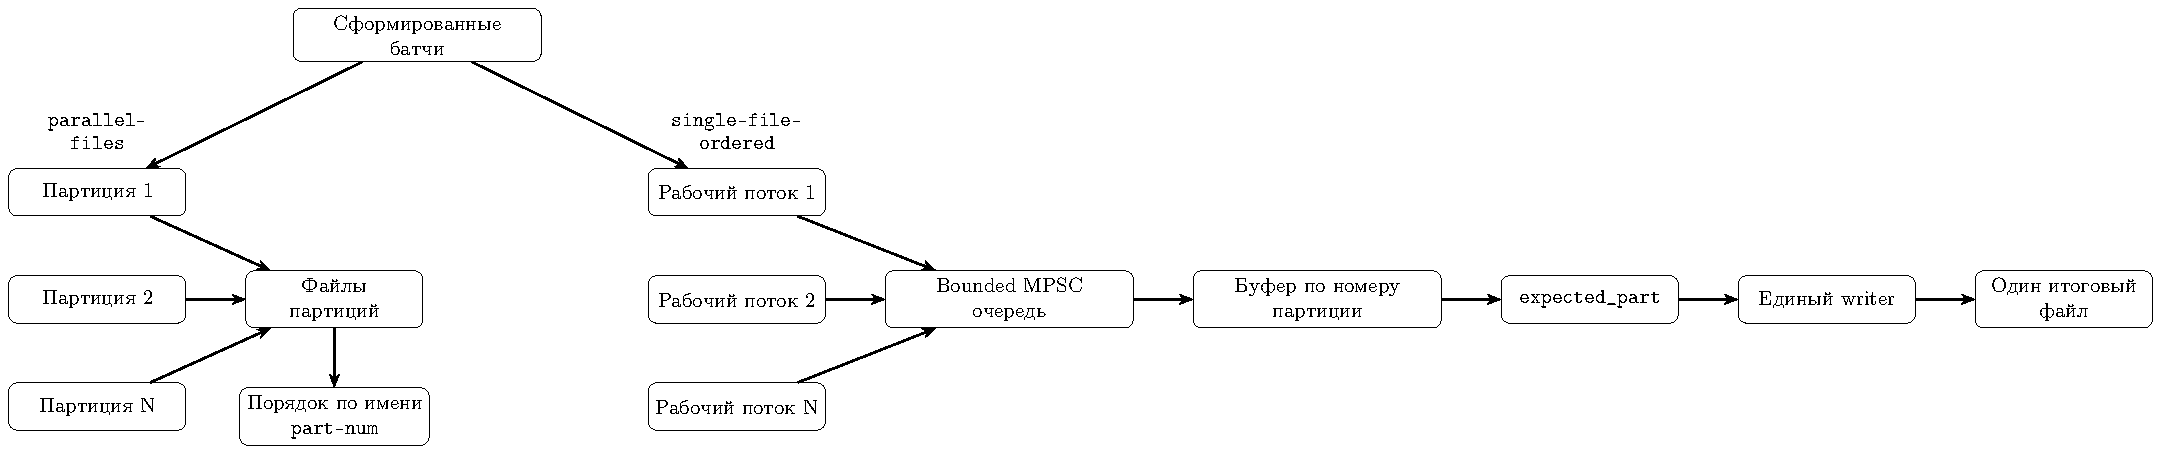
\includegraphics[width=\textwidth]{../expl-note/image/serialization-diagram.pdf}
\caption{Схема ручного упорядочения партиций для форматов с управляемым стримингом}
\label{fig:chapter3-serialization-diagram}
\end{figure}

\begin{lstlisting}[style=reportpseudocode,caption={Упорядоченная запись в один итоговый файл},label={lst:chapter3-ordered-write}]
func write_ordered_single_output(table, batches, output_format):
    expected_part = 1
    buffered_parts = {}

    for message in batches:
        buffer_message(buffered_parts, message)
        flush_ready_partitions(buffered_parts, expected_part, output_format)
\end{lstlisting}

Такое решение позволяет совместить параллельную генерацию батчей с линейным
порядком данных в итоговом файле. Именно этот механизм обеспечивает одинаковый
логический порядок результата независимо от конфигурации рабочих потоков.

\subsubsection{Форматы с нативным стримингом}

Для форматов Lance~\cite{lance-format} и
Vortex~\cite{vortex-format} реализован другой сценарий: система
последовательно передает уже сформированные батчи во внешний форматный рантайм.
Тем самым генератор отвечает за границы партиций и порядок передачи
данных, а физическое размещение и внутренняя структура набора данных
определяются библиотекой соответствующего формата.

\begin{lstlisting}[style=reportpseudocode,caption={Передача батчей во внешний рантайм формата},label={lst:chapter3-foreign-runtime}]
func stream_to_native_runtime(table, batches, output_format):
    runtime = open_runtime(output_format, table.schema)

    for partition in batches:
        runtime.begin_partition(partition.number)

        for batch in partition.batches:
            runtime.push_batch(batch)

    runtime.finish()
\end{lstlisting}

\subsection{Интерфейс запуска и сценарии эксплуатации}

\subsubsection{Параметры командной строки}

Интерфейс запуска построен вокруг параметров командной строки. Пользователь
может получить справку, вывести перечень таблиц, выбрать формат хранения,
стратегию записи, каталог вывода и набор таблиц, которые необходимо
сгенерировать. Фактический перечень доступных форматов зависит от активных
драйверов текущей сборки.

\begin{table}[H]
\caption{Основные параметры командной строки}
\label{tab:chapter3-cli-options}
\centering
\small
\begin{tabularx}{\textwidth}{|p{0.28\textwidth}|X|}
\hline
\textbf{Параметр} & \textbf{Назначение} \\
\hline
\texttt{--help} & Вывод справки по параметрам запуска. \\
\hline
\texttt{--list-tables} & Вывод списка поддерживаемых таблиц TPC-H. \\
\hline
\texttt{--list-formats} & Вывод форматов, доступных в текущей сборке. \\
\hline
\texttt{--scale-factor} & Задание масштаба генерации. \\
\hline
\texttt{--output-format} & Выбор целевого формата хранения. \\
\hline
\texttt{--output-path} & Путь или URI каталога вывода. \\
\hline
\texttt{--table} & Перечень таблиц для генерации; при отсутствии параметра формируются все таблицы. \\
\hline
\texttt{--batch-rows} & Максимальное число строк в одном батче. \\
\hline
\texttt{--write-strategy} & Выбор стратегии записи: \texttt{auto}, \texttt{parallel-files}, \texttt{single-file-ordered}. \\
\hline
\texttt{--write-workers} & Число рабочих потоков обработки партиций, \texttt{0} означает автоматический выбор. \\
\hline
\texttt{--write-queue-capacity} & Емкость очереди батчей при упорядоченной записи. \\
\hline
\texttt{--verbosity} & Режим вывода хода выполнения: \texttt{quiet} или \texttt{verbose}. \\
\hline
\end{tabularx}
\normalsize
\end{table}

Помимо общих параметров, драйверы форматов добавляют собственные группы
настроек: параметры сжатия, размеры буферов и ограничения на размер
форматно-зависимых блоков хранения. В практическом использовании это позволяет
не изменять общий интерфейс запуска при добавлении нового драйвера или новой
стратегии записи.

\subsubsection{Типовые сценарии запуска}

Типовые сценарии эксплуатации приведены в листинге
\ref{lst:chapter3-cli}. Они охватывают получение служебной информации,
генерацию нескольких таблиц, запись в единый файл и сохранение данных по
URI.

\begin{lstlisting}[style=reportlisting,caption={Примеры запуска генератора},label={lst:chapter3-cli}]
schengen_main --help

schengen_main --list-formats

schengen_main \
  --scale-factor 10 \
  --output-format parquet \
  --output-path ./out \
  --table customer orders lineitem

schengen_main \
  --scale-factor 10 \
  --output-format orc \
  --output-path ./out_orc \
  --write-strategy single-file-ordered \
  --write-workers 4

schengen_main \
  --scale-factor 10 \
  --output-format lance \
  --output-path s3://bucket/tpch \
  --table lineitem
\end{lstlisting}

Структура выходных данных определяется сочетанием формата и стратегии записи.
При использовании раздельной записи партиций каталог таблицы содержит набор
файлов-партиций. В режиме упорядоченной записи в один файл внутри каталога таблицы
создается один итоговый артефакт. Такая организация позволяет единообразно
адресовать результат по схеме \texttt{<output>/<table>/<artifact>}.

\subsection{Реализация встраиваемого сценария}

\subsubsection{Идея встроенного сценария}

Отделение генератора от слоя сериализации позволяет использовать его не только
как автономную утилиту записи файлов, но и как источник табличных данных для
аналитической СУБД. В таком сценарии сгенерированные в оперативной памяти
батчи передаются непосредственно в движок OLAP-системы, минуя запись
на диск, последующее чтение файлов, декодирование формата хранения и другие
накладные расходы, характерные для файлового конвейера.

Практическая ценность этого варианта состоит в том, что генератор можно
встраивать в систему исполнения запросов и использовать для моделирования
нагрузки без предварительной материализации набора данных. Тем самым одна и та
же реализация пригодна и для подготовки колонoчных файлов, и для прямой
подачи синтетических таблиц во внутренний движок СУБД.

\subsubsection{Демонстрационный прототип для DuckDB}

В качестве демонстрационного \textit{proof-of-concept} такой сценарий
реализован в виде отдельного расширения для DuckDB
~\cite{schengen-duckdb-repo,duckdb-extensions}. Выбор именно этой СУБД
обусловлен удобной инфраструктурой пользовательских расширений и сравнительно
простой схемой подключения внешних табличных источников. Это позволяет
проверить саму возможность интеграции генератора в аналитическую систему без
существенной перестройки ядра генерации.

В расширении генераторная часть используется напрямую, без слоя сериализации.
Пользователю доступны вызов \texttt{CALL schengen(scale\_factor)} для
публикации временных представлений и табличная функция
\texttt{schengen\_scan}, возвращающая одну выбранную таблицу. С точки зрения
архитектуры этот прототип показывает, что генератор может работать как
встроенный компонент СУБД и поставлять данные непосредственно в исполнитель
запросов, не проходя через промежуточные форматы хранения.

\begin{lstlisting}[style=reportlisting,caption={Использование встроенного сценария через DuckDB},label={lst:chapter3-duckdb}]
LOAD schengen;
CALL schengen(1);

SELECT COUNT(*) FROM lineitem;
SELECT * FROM schengen_scan('orders', 1) LIMIT 5;
\end{lstlisting}

\subsection*{Выводы по главе}
\addcontentsline{toc}{subsection}{Выводы по главе}

В третьей главе показано, как архитектурные решения предыдущей главы
реализованы в программной системе. Генератор построен вокруг отдельных
модулей формирования таблиц, общего текстового пула и колонoчного
представления Apache Arrow. Слой сериализации поддерживает несколько
форматов хранения и две основные стратегии записи.

Также показано, что отделение ядра генерации от слоя сериализации позволило
реализовать встраиваемый сценарий с DuckDB, в котором те же батчи
используются без промежуточной записи на диск. Тем самым генератор
поддерживает как автономную файловую эксплуатацию, так и внутрипамятную
интеграцию с аналитической СУБД.
